\documentclass[../../main.tex]{subfiles}
\begin{document}

\begin{flushright}
  \footnotesize\textit{【自動文字起こし・要確認】}
\end{flushright}

% Source: handwritten.pdf 第4問．
{\bf [解答]}
$AB=a$，$AC=b$，$BC=\sqrt{3}$とし，外心をOとする．鋭角三角形なのでOは三角形の内部にある．$OB=OC=1$より
\begin{align}
  \angle BOC=\dfrac{2\pi}{3},\qquad \angle BAC=\dfrac{\pi}{3}.
\end{align}
余弦定理によって
\begin{align}
  3&=a^2+b^2-2ab\cdot\dfrac{1}{2}=a^2+b^2-ab,\\
  b&=\dfrac{a\pm\sqrt{12-3a^2}}{2}.
\end{align}
% 原稿の「複号負はb<0」を転記．sqrt(3)<a<2ではこの符号判定は成立せず，要確認．
$1<a<2$より負号の場合は$b<0$となるので不適．したがって
\begin{align}
  b=\dfrac{a+\sqrt{12-3a^2}}{2}.
\end{align}
\begin{figure}[H]
  \centering
  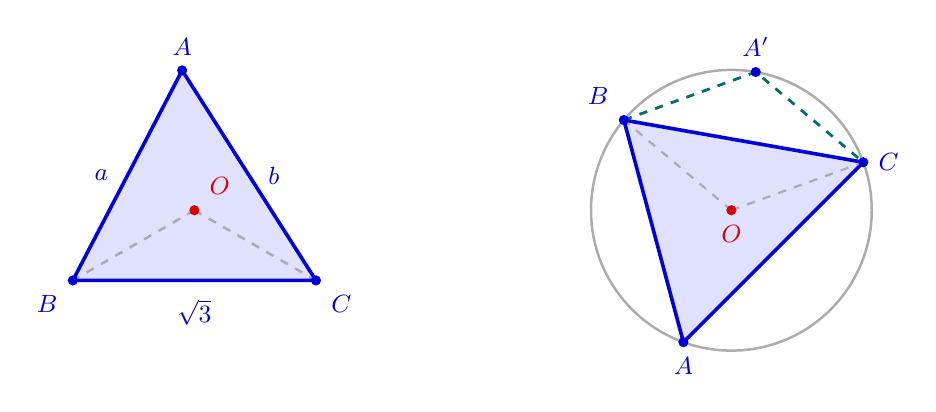
\begin{tikzpicture}[scale=1.55, >=stealth, every node/.style={font=\small}]
    % 左：鋭角三角形，右：短い弧 BC 上の A' では角 BA'C が鈍角となる．
    \begin{scope}
      \coordinate (O) at (0,0);
      \coordinate (A) at (95:1.15);
      \coordinate (B) at (210:1.15);
      \coordinate (C) at (330:1.15);
      \fill[blue!12] (A)--(B)--(C)--cycle;
      \draw[dashed, gray!65, line width=0.9pt] (O)--(B) (O)--(C);
      \draw[blue!85!black, line width=1.3pt] (A)--(B)
      node[midway, left=3pt] {$a$}
      --(C) node[midway, below=3pt] {$\sqrt{3}$}
      --(A) node[midway, right=3pt] {$b$};
      \node[circle, fill=red!85!black, inner sep=1.3pt] at (O) {}; \node[red!85!black, above right=2pt] at (O) {$O$};
      \foreach \point/\position in {A/above,B/below left,C/below right} {
        \node[circle, fill=blue!85!black, inner sep=1.3pt] at (\point) {}; \node[blue!85!black, \position=2pt] at (\point) {$\point$};
      }
    \end{scope}
    \begin{scope}[xshift=4.4cm]
      \coordinate (O2) at (0,0);
      \coordinate (A2) at (250:1.15);
      \coordinate (B2) at (140:1.15);
      \coordinate (C2) at (20:1.15);
      \coordinate (Aprime) at (80:1.15);
      \draw[gray!65, line width=0.9pt] (O2) circle (1.15);
      \fill[blue!12] (A2)--(B2)--(C2)--cycle;
      \draw[blue!85!black, line width=1.3pt] (A2)--(B2)--(C2)--cycle;
      \draw[dashed, teal!85!black, line width=1pt] (B2)--(Aprime)--(C2);
      \draw[dashed, gray!65, line width=0.8pt] (O2)--(B2) (O2)--(C2);
      \node[circle, fill=red!85!black, inner sep=1.3pt] at (O2) {}; \node[red!85!black, below=2pt] at (O2) {$O$};
      \foreach \point/\position/\name in {
      A2/below/$A$, B2/above left/$B$, C2/right/$C$, Aprime/above/$A'$} {
        \node[circle, fill=blue!85!black, inner sep=1.3pt] at (\point) {}; \node[blue!85!black, \position=2pt] at (\point) {\name};
      }
    \end{scope}
  \end{tikzpicture}
  \caption{鋭角三角形$ABC$の外心$O$と円周角の位置関係}
\end{figure}

\end{document}
